\subsection*{Paikkajärjestelmät}

Merkitsemme lukuja yleensä kymmenjärjestelmässä eli lukujärjestelmässä, jossa on kymmenen numeromerkkiä: $0, 1, 2, 3, 4, 5, 6, 7, 8, 9$.
\footnote{Muitakin numeromerkkejä voisi käyttää. Käyttämämme numeromerkit ovat nimeltään hindu-arabialaiset numerot.}
Kymmenjärjestelmä tunnetaan myös desimaalijärjestelmänä. Tiedämme kuitenkin kulttuureja, joissa on käytetty pääasiallisesti jotakin muuta lukujärjestelmää.

Kymmenjärjestelmä on paikkajärjestelmä, eli merkin paikka määrittää sen merkityksen. Esimerkiksi luvussa $80$ merkin 8 merkitys on $8 \cdot 10^1$, mutta luvussa
$820$ sen merkitys on $8 \cdot 10^2$.

Nykyään yleisimmät desimaalijärjestelmästä poikkeavat lukujärjestelmät ovat binääri-, oktaali- ja heksadesimaalijärjestelmät, joissa on 2, 8 ja 16 numeromerkkiä.
Tietokoneet käsittelevät lukuja sisäisesti binäärijärjestelmässä, kun taas oktaali- ja heksadesimaalijärjestelmät ovat muutoin käteviä tietojenkäsittelytieteessä.

Binäärijärjestelmässä luvun muodostavia numeromerkkejä kutsutaan biteiksi.
Bitti voi olla joko päällä (1) tai pois päältä (0), ja toteutus tietokoneessa vastaa esimerkiksi sitä, että johtimessa kulkee virta (1) tai ei (0).

Kuusitoistajärjestelmässä tarvitaan numeroiden $0 \ldots \, 9$ lisäksi kuusi uutta numeromerkkiä.
Tavaksi on vakiintunut käyttää kirjainmerkkejä $\mathrm{A, B, C, D, E, F}$. Ne vastaavat desimaalilukuja $10 \ldots \, 15$.

Useampaa järjestelmää käytettäessä, erityisesti muunnettaessa lukuja järjestelmästä toiseen, merkitään kantaluku luvun jälkeen alaindeksinä.
Voimme esimerkiksi merkitä (desimaalijärjestelmän) lukua yhdeksäntoista $10011_{2}$, $23_{8}$, $19_{10}$ tai $13_{16}$.

Lukujärjestelmiä voidaan vaihtoehtoisesti merkitä kirjoittamalla niiden tunnus (Bin, Oct, Dec, Hex) luvun jälkeen.
Klassinen vitsi ''Miksi tietojenkäsittelytieteilijä sekoittaa halloweenin ja joulun? Koska 31 Oct = 25 Dec!'' perustuu siihen, että

\begin{align*}
	\text{halloween} \; = \; \text{31. lokakuuta} \; &= \; \text{31 Oct} \; = 31_8 = 3_{10} \cdot 8_{10} + 1_{10} \cdot 1_{10} \\
	= {25}_{10} &= \; \text{25 Dec} \; = \; \text{25. joulukuuta} \; = \; \text{joulupäivä.}
\end{align*}

\subsection*{Muut lukujärjestelmät}

Yleisesti tunnetaan myös joitakin lukujärjestelmiä, jotka eivät ole paikkajärjestelmiä.

Tukkimiehen kirjanpidossa toistetaan yhtä ainoaa merkkiä. Se on tavallaan 1-järjestelmä, mutta tällainen määrittely ei ole ongelmaton.

\begin{center}
	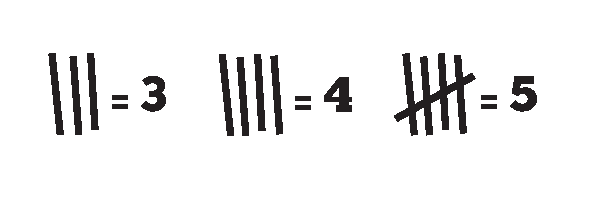
\includegraphics{pictures/Kuva1-1-tukkimiehenkirjanpito.pdf}
\end{center}

Hienostuneempi versio tukkimiehen kirjanpidosta on roomalaiset luvut, jotka nimensä mukaisesti olivat antiikin Roomassa keskeisin lukujärjestelmä.
Ne perustuvat havaintoon, että kun käytettävissä olevien merkkien määrää lisää, suuria lukuja voi kirjoittaa lyhyempään muotoon.
Tilanne on verrattavissa vaikkapa kiinan kieleen, jossa on käytössä satoja erilaisia kirjoitusmerkkejä.
Merkeissä on paljon muistettavaa, mutta toisaalta kokonaisen lauseen voi kirjoittaa vain parilla kirjoitusmerkillä.

Roomalaisia lukuja käytetään yhä nykyäänkin erityisesti järjestyksen merkitsemisessä.

Roomalaisten lukujen numeromerkit ovat I, V, X, L, C, D ja M. Ne vastaavat desimaalijärjestelmän lukuja seuraavalla tavalla:

\begin{equation*}
	\rm I=1\quad
	V=5\quad
	X=10\quad
	L=50\quad
	C=100\quad
	D=500\quad
	M=1~000
\end{equation*}

Roomalaiset luvut merkitään kirjoittamalla merkkejä laskevassa järjestyksessä, poikkeuksena vähennyssääntö. Merkkien kokonaisarvo määrää luvun.

Lisäksi on kuusi kaksimerkkistä ilmaisua, jotka tunnetaan myös vähennyssääntönä: IV = $4$, IX = $9$, XL = $40$, XC = $90$, CD = $400$ ja CM = $900$.
Niistä kukin voi esiintyä luvussa vain kerran. Kaksimerkkisiin ilmaisuihin pätevät samat säännöt kuin numeromerkkeihinkin:
I = $1$ ei voi edeltää numeroa IV = $4$, eikä IV = $4$ numeroa V = $5$. Lisäksi merkinnät IXV, XCL ja CMD eivät ole sallittuja.

Oikea roomalainen luku minimoi käytettyjen merkkien määrän. Esimerkiksi VIV ei ole roomalainen luku, sillä IX on lyhyempi.

Nollaa roomalaisissa numeroissa ei ole; nolla nykyisessä merkityksessään kehitettiin Intiassa 800-luvulla jaa.

\begin{esimerkki}
	Roomalaisia lukuja:
	\begin{alakohdat}
		\alakohta{III$=1+1+1=3$}
		\alakohta{IX$=10-1=9$}
		\alakohta{XII$=10+1+1=12$}
		\alakohta{XIV$= 10 + (5 - 1) = 14$}
		\alakohta{CDX$=500-100+10=410$}
		\alakohta{MDC$=1 000+500+100=1~600$}
	\end{alakohdat}
\end{esimerkki}

\subsection*{Huomautuksia}

Numero ja luku eivät ole synonyymejä; numero on yksittäinen lukujärjestelmän merkki.

\begin{esimerkki}
	Luku \[715531\] koostuu numeroista 7, 1, 5, 5, 3 ja 1.
	Luku \[9\] koostuu ainoastaan vastaavasta numeromerkistä 9.
\end{esimerkki}

Englannin kielen sana \textit{number} voi viitata sekä numeroon että lukuun.
Sana \textit{digit} tarkoittaa pelkästään yhtä numeromerkkiä.
Ruotsiksi luku on \textit{tal}, lukumäärä \textit{antal} ja numeroa tai lukumäärää tarkoittamatonta numeroyhdistelmää kuvaa suomen kielen tapaan sana \textit{nummer}.

Luvulla on aina suuruus mutta numerolla ei välttämättä ole. Esimerkiksi arkipäivän käsitteet postinumero ja puhelinnumero eivät ole lukuja, vaikka niissä numeroita yhdistelläänkin. 
Emme voi esimerkiksi sanoa, onko postinumero 00950 jollakin tapaa suurempi kuin postinumero 00900.

Tuhaterottimena käytetään suomenkielisessä tekstissä välilyöntiä, ei pilkkua tai pistettä.
Desimaalierotin puolestaan on suomenkielisessä tekstissä pilkku, ei piste, kuten yhdysvaltalaisissa laskimissa.
